% Chapter 2


\chapter{PROPOSED METHODOLOGY}

% -----------------------------------------
% 3.1 ARCHITECTURE DESIGN (CONTENT ONLY – FULL PAGE)
% -----------------------------------------

\section{ARCHITECTURE DESIGN}

The system architecture is developed in such a way that it can handle the incoming data in various batches and update the feature representation dynamically for efficient social engineering attack detection. The system starts with a series of data batches, in which every batch goes through a Feature Updation phase. This module is tasked with the responsibility of preparing and optimizing the input data by using various preprocessing techniques such as cleaning, normalization, transformation, and extraction of key attributes. As the system receives the data in batches and not a static dataset, the Feature Updation module is used to process every batch independently and transform it into a new feature set as illustrated in Fig~\ref{fig:architecture}

Once the feature updation process is completed, the updated features are passed to the Neural Network Module. The Neural Network Module is the central part of the architecture and is tasked with learning the discriminative patterns from the updated features and developing models for classification. As evident from the architecture, each batch is used to develop a model that is referred to as $M_1$, $M_2$, $M_3$, and so on.

\begin{figure}[H]
\centering
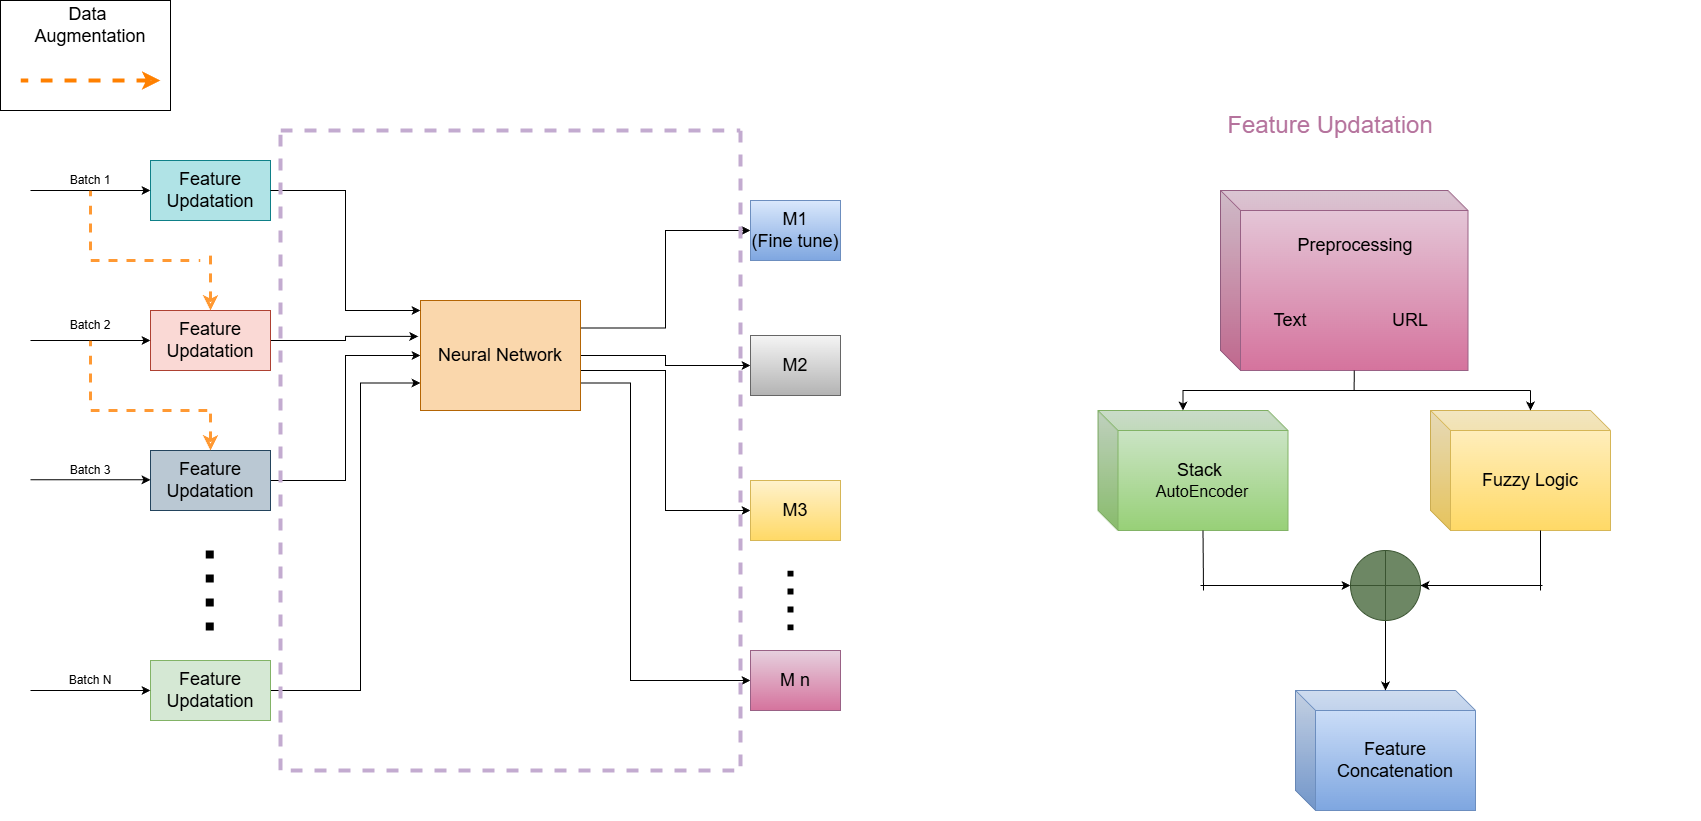
\includegraphics[width=\textwidth]{images/Review2_architecture.drawio.png}
\caption{Architecture Design of Proposed System}
\label{fig:architecture}
\end{figure}

In parallel to the process of updating features in batches, there is also a Data Augmentation module in the system that introduces diversity and variability to the training data. Whether it is the creation of new data samples synthetically or the creation of new samples from the existing ones, the data augmentation module is responsible for enhancing the generalization capability of the neural network as well as ensuring that it does not overfit. The process of updating features in batches and data augmentation ensures that the learning process remains stable even when the input batches have different distributions and structures.

On the right side of the architecture, the internal workflow of the Feature Updation Module has been shown in more detail. The Preprocessing module processes two types of data, Text and URL, thereby ensuring that both types of data are properly preprocessed. The preprocessed data is then fed to a Stacked Autoencoder, which reduces the dimensionality of the data and extracts meaningful latent features. Along with the autoencoder, a Fuzzy Logic module is used to process the uncertainties and linguistic nuances that are present in the data. The output of both the autoencoder and the fuzzy logic module is then combined using a Feature Concatenation module, resulting in a homogeneous feature vector that is then fed to the neural network for training and model development.

Overall, the architecture is designed to enable continuous learning, multi-modal feature refinement, and incremental model synthesis. By integrating preprocessing, fuzzy logic processing, stacked autoencoder-based feature extraction, and batch-based neural learning, the architecture provides a well-organized and scalable data pipeline from raw data to the final attack prediction.



\section{ELM Based Classification Architecture} 

The architecture of the system is designed to detect social engineering attacks by analyzing two different types of input data, which are text and URL features, by combining them into a single feature space. The system begins with the Data Loading module, where the data set containing the two types of input data is loaded into the system. Once the data is loaded, it is divided into its respective components and then sent to the two preprocessing paths.

The Text Preprocessing module performs operations such as text cleaning, lemmatization, removal of noise, and transformation into numerical vector form using TF-IDF vectorization followed by Truncated SVD for dimensionality reduction. The URL Preprocessing module extracts structural and lexical characteristics from the raw URL strings — including URL length, dot count, slash count, HTTPS presence, and character-level n-gram TF-IDF features — normalizes the values, and prepares them for feature learning.

After preprocessing, each data modality is sent to its corresponding Stacked Autoencoder (SAE) component — SAE Text and SAE URL. These autoencoders reduce the dimensionality of the processed inputs and learn meaningful latent feature representations. Instead of manually selecting features, the stacked autoencoders automatically extract hidden patterns and compress the information while preserving the critical characteristics of each data type. The text autoencoder follows a 200 → 100 → 50 → 100 → 200 architecture, producing a 50-dimensional encoded text representation, while the URL autoencoder follows a 68 → 60 → 50 → 60 → 68 architecture, producing a 50-dimensional encoded URL representation. Both the autoencoders are trained only on the Day 1 data, and their weights are frozen for the rest of the days. This ensures that the feature space is stable throughout the learning process.

The encoded outputs are then combined in the Combined Feature module. The Combined Feature module utilizes feature-level combination by concatenating the two 50-dimensional latent outputs into a combined 100-dimensional feature vector from Pipeline 1. Simultaneously, the Fuzzy-PGFDG module from Pipeline 2 generates a second 24-dimensional feature vector that encompasses 19 manual text and URL features expanded with 5 fuzzy descriptors: Typicality, Density, Homogeneity, Outlier Score, and Fuzzy Entropy. The output from Pipeline 1 and Pipeline 2 is then concatenated to generate the final 124-dimensional combined feature vector that encompasses a broad spectrum of information from both deep autoencoder latent outputs and fuzzy interpretable features.

This combined 124-dimensional feature vector is then fed into the Extreme Learning Machine (ELM) classifier. The ELM is a single-hidden-layer feedforward neural network that trains much faster than backpropagation-based models. The weights and biases of the hidden layer of the ELM are randomly generated and then fixed, and the output weights are determined in a single step using the Moore-Penrose pseudoinverse.

Finally, the trained ELM predicts the attack type using the combined 124-dimensional feature input. The ELM classifies each input instance into one of five categories: Baiting, Legitimate, Phishing, Pretexting, or Whaling. The ELM model of the previous day is intentionally deleted after each update, and only the new ELM model is saved, which ensures that the memory usage remains bounded for all incremental days. In conclusion, the architecture provides a systematic and optimized workflow from data loading to attack prediction, which covers preprocessing, automatic deep feature extraction, fuzzy feature generation, feature fusion, and analytically derived incremental classification.

\section{MODULES}
The proposed system is designed using a modular approach, where each module is designed to serve a distinct and critical purpose in the entire process of social engineering attack detection. The proposed system deals with two different types of data: textual content and URL features. Therefore, the proposed system consists of distinct modules designed specifically to deal with each type of data in an effective manner. The process begins with the Data Loading module, which loads the dataset and organizes it in the required formats. This module ensures that all the data is organized in the required and separated into text and URL components so that the subsequent stages receive clean and well-organized inputs.

Once the data is loaded, it is then passed through the Preprocessing module, which is tasked with the responsibility of preparing the data for further processing. Since each modality has its own unique features, two preprocessing pipelines are used. The text preprocessing entails the cleaning, tokenization, and vectorization of the raw text data, which makes it possible to transform the raw text data into numerical form. The URL preprocessing entails the extraction of structural and lexical features that help in the identification of malicious link patterns.

The processed data is then passed on to the Stacked Autoencoder (SAE) module. The SAE module is a very important part of the process of extracting significant hidden features from each type of data. Rather than using feature engineering, which is a time-consuming process, autoencoders are used to automatically extract hidden patterns and reduce the high-dimensional input into a lower-dimensional space. Autoencoders are employed independently for text data as well as URL modalities, ensuring that each type of data is mapped to its features based on its structural properties.

The output of the two autoencoders is merged in the Combined Feature module, where the combination of features at the feature level is performed. This module combines the latent features of all the modalities into a single feature representation. By combining the information from the text, URL data, the system obtains a better understanding of the samples, which helps in accurately identifying the attack patterns. The combined feature vector is the final input to the classification models.

The Classification module consists of one neural network model: Extreme Learning Machine (ELM). That model use the fused feature vector to predict the attack type. ELM uses randomly generated hidden nodes to train quickly.Model can be used to distinguish benign data from different types of social engineering attacks.

Finally, the Output module relays the result of the prediction to the user by specifying the attack category that has been identified. The modular structure of the system from data loading to preprocessing, feature learning, feature fusion, classification, and finally to output ensures that the system is efficient and scalable enough to handle multi-modal inputs for attack detection.

\subsection{Data Loading}
The Data Loading process is the backbone of the entire detection system because it is responsible for the importation, organization, and proper structuring of all the data used in the entire process. In this project, the data consists of two forms of information: text information and URL-related information. Because both forms of information have different properties, the Data Loading module is responsible for ensuring that both forms of information are properly identified and separated for the next modules to handle them in the correct manner.

When the data set is received, it starts with the process of reading the input from its source, such as CSV files, and validating the integrity of the data. It makes sure that there are no missing fields, that the data types are not incorrect, and that the formatting is consistent. The process also validates the number of samples, the alignment of the labels with the features, and breaks down the content into two structured parts. The text fields are stored in a separate structure so that they can be further preprocessed linguistically. The URL strings are stored in a separate area, awaiting URL-specific type extraction and cleaning.

Another significant task related to this step is the handling of errors and anomalies that are present in the raw data. These can be in the form of blank entries, incorrect entries, noisy symbols, or broken lines. The Data Loading is tasked with the preliminary filtering of the data to remove or point out erroneous data. In some cases, it is also tasked with documenting any discrepancies for later review, as a way of promoting transparency and debugging.

By the time the data loading process is completed, the system will have a well-structured format of text and URL, data. This is an important aspect because it will ensure that all the preprocessing modules receive the data in the exact format that they require.The Data Loading process is important because it will ensure the stability, reliability, and correctness of all the input data.

\subsection{Preprocessing Module}
The Preprocessing Module is a crucial component of the proposed system, as it attempts to transform the raw and unstructured inputs into clean, meaningful, and machine-readable formats. Considering the fact that the dataset comprises two distinct types of data: text and URL attributes, the preprocessing module comprises two distinct preprocessing pipelines. The two preprocessing pipelines are designed in such a manner that they are capable of handling the nature of their respective data modalities. The preprocessing module ensures that noise is eliminated, inconsistencies are resolved, and all data formats are transformed into structured formats that are ready for processing and feature extraction. The preprocessing module will ultimately be responsible for preparing the data for the Stacked Autoencoder and neural classification models.

\subsubsection{Text Preprocessing}

The Text Preprocessing is concerned with the cleaning and normalization of the text data acquired from posts, messages, or descriptions available on social media platforms. The raw text data usually comprises unnecessary characters, emojis, URLs, repeated symbols, case variations, and unnecessary stopwords that do not add any value to the meaningful information. This module is responsible for the cleaning of the text data by eliminating all the unnecessary characters and normalizing the text. The process starts with the conversion of text to lowercase to ensure consistency, followed by the removal of special characters, punctuation, and unnecessary spaces. The tokenization process is then used to split the sentences into individual words or meaningful pieces. Stemming or lemmatization is used to convert words to their root form to eliminate redundancy in the vocabulary.

After the cleaning process is finished, the text data must be converted into a form of numbers that can be handled by machine learning algorithms. A technique commonly employed for this task is {TF-IDF (Term Frequency-Inverse Document Frequency)}, which gives more significant to important words and reduces the effect of frequently occurring words. The TF-IDF value of a word $t$ in a document $d$ is given by the following formula:

\begin{equation}
\label{Eq1}
\text{TF-IDF}(t, d) = \text{TF}(t, d) \times \log\left( \frac{N}{\text{DF}(t)} \right)
\end{equation}


where,
\begin{itemize}
    \item $\text{TF}(t,d)$ is the frequency of term $t$ in document $d$,
    \item $N$ is the total number of documents, and
    \item $\text{DF}(t)$ is the number of documents containing term $t$.
\end{itemize}

This formula gives higher importance to terms that are frequent in one document but rare across others. In the context of attack detection, TF--IDF helps highlight contextual keywords and suspicious linguistic patterns often found in phishing, impersonation, or malicious messages.

However, TF--IDF vectors are often very high-dimensional, which can slow down the learning process and reduce model efficiency. To reduce dimensionality while preserving the essential meaning of the text,{Singular Value Decomposition (SVD)} is applied to the TF--IDF matrix. Mathematically, the decomposition is expressed as:

\begin{equation}
\label{Eq1}
X_{\text{TF-IDF}} = U \Sigma V^{T}
\end{equation}


where,
\begin{itemize}
    \item $U$ captures document-level patterns,
    \item $\Sigma$ contains the most important ``strengths'' or weights of the patterns, and
    \item $V^{T}$ represents word-level relationships.
\end{itemize}

That is, SVD helps in reducing the TF-IDF matrix, which is quite large, to its most significant components, so that the system can focus on the most significant linguistic aspects while ignoring the rest.

By carrying out the above-mentioned steps of cleaning, normalization, number conversion, and dimensionality reduction. The Text Preprocessing module ensures that only the most significant and compact representation of the text features are passed on to the feature extraction stage.

\subsubsection{URL Preprocessing}
The URL Preprocessing is intended to identify valuable structural and lexical patterns from the links of websites. URLs are known to hold important features of malicious activities, since attackers tend to incorporate deceptive components to deceive users. To identify these features, the preprocessing process tends to evaluate various components of each URL, including domain names, subdomains, path formats, query strings, and encoded characters. Features such as URL length, the number of numeric characters, the number of special characters, the presence of deceptive keywords, the use of HTTPS, or the presence of IP domain names are extracted and analyzed. Other lexical features might include character frequency patterns or entropy values. 

After feature extraction, the values of these features are normalized to maintain numerical consistency for all samples. This is done to make the machine learning model consider all features equally. The normalization process is carried out using the Standard Scaler as follows:

\begin{equation}
X_{\text{norm}} = \frac{X - \mu}{\sigma}
\end{equation}

where \(X\) is the original feature value, \(\mu\) is the mean of the feature across all samples, and \(\sigma\) is the standard deviation. This transformation ensures that features with larger numerical ranges do not dominate those with smaller ranges, improving model performance and stability.

The resulting cleaned and structured URL features help the system distinguish between normal links and deceptive or malicious URLs, significantly contributing to accurate attack detection.


\subsection{Stacked Autoencoder (SAE) Module}
The Stacked Autoencoder (SAE) module is given the task of extracting hidden patterns from the preprocessed data and then reducing the dimensionality of the data while preserving the crucial information. Since the system handles two different types of inputs, namely text and URL, two different autoencoders are used: SAE Text and SAE URL. Both autoencoders are trained separately to extract the important hidden patterns based on their respective data types.

\subsubsection{SAE Text Module}
The purpose of the SAE Text module is to reveal the hidden patterns in the linguistic and semantic structures from the preprocessed text data. The text data is expected to have complex patterns, word relations, and hidden semantic information that are difficult to model using simple and manually designed features. The SAE Text module automatically discovers the patterns by compressing the input text using multiple layers, creating a latent space that captures the essential characteristics of the text.

In the encoding process, the input text is compressed step by step, and each layer learns to capture the essential relations among words, phrases, or context-dependent features. To introduce non-linearity and allow the network to model complex relations, {LeakyReLU activation} is used in the hidden layers. The LeakyReLU activation function is defined as:

\begin{equation}
\text{LeakyReLU}(x) =
\begin{cases} 
x, & \text{if } x > 0 \\
\alpha x, & \text{if } x \le 0
\end{cases}
\end{equation}

where \(\alpha = 0.2\). This activation allows small negative values to pass through instead of setting them to zero, preventing neurons from becoming inactive and helping the network learn more robust representations.

The encoding process results in a compact vector representation that encodes the semantic essence of the text. The decoding process is tasked with the responsibility of recovering the original input from the latent vector, ensuring that the compressed vector is semantically meaningful. Although the reconstructed text is not used in the system, this process ensures that the latent vector preserves the most important aspects of the text.

SAE Text reduces noise and redundancy by converting raw text into dense vectors, hence reducing the dimensionality of the input data. The representation form of the input data is of high quality and is an ideal input for the classifiers, which can easily classify the malicious content. SAE Text automates the feature extraction process of the input text data.


\subsubsection{SAE URL Module}
The SAE URL module is concerned with learning structural and behavioral patterns from URL data. URLs are known to have indicators of potential attacks, including suspicious subdomains, path patterns, query strings, and encoded characters. The SAE URL module is able to learn these patterns by compressing the URL features into latent vectors.

During the encoding process, the module gradually decreases the dimensionality of the URL features, learning the relationships between structural elements, character distributions, and other lexical features. The latent vector learned from this process captures the behavior of the URL, making it easier for classifiers to distinguish between malicious and benign behavior. During the decoding process, the input URL is reconstructed to ensure that the key information is captured in the compressed form.

The SAE URL module removes unnecessary information, focusing only on the information that is crucial in making a distinction between normal and malicious URLs. The SAE URL module enhances the performance of the MLP and ELM classifiers by producing high-quality compact vectors. This module ensures that the system is able to process a large amount of URL information while still being accurate in attack detection.

\subsection{Combined Feature Module}
The Combined Feature module is a feature-level fusion module where the latent features extracted from the two Stacked Autoencoders are combined. Once each modality, text, and URL, has been represented as a compact feature vector, the vectors are combined to represent the input instance. This is an important step in the process as it enables the system to process both types of input simultaneously, thus enhancing its capability to identify complex attack patterns.

The concatenation of the latent vectors can be represented as:

\begin{equation}
X_{\text{fused}} = X_{\text{bottleneck}}^{\text{text}} \; \| \; X_{\text{bottleneck}}^{\text{url}} \; \| \; 
\end{equation}

where \(X_{\text{bottleneck}}^{\text{text}}\)and \(X_{\text{bottleneck}}^{\text{url}}\)are the latent vectors obtained from the SAE Text, SAE URL, and SAE Tabular modules, respectively. The symbol \(\|\) denotes vector concatenation. This step simply concatenates the three vectors together, forming a single unified feature vector that aggregates information from all three modalities. In doing so, the classifier is provided with a more informative representation of each sample, one that aggregates individual and cross-modal patterns.

The module also maintains structural consistency of the aggregated vector for all samples by addressing feature alignment, dimension consistency, and order. This structured unified representation serves as the input to the neural classifiers, allowing them to make more informed decisions. For instance, a phishing attack may contain suspicious text features, irregular URL features, and irregular metadata features; when all three modalities are aggregated, the system is able to identify these patterns more effectively.

The Combined Feature module consolidates multi-modal latent features into a single structured vector, enhancing the system’s predictive power and supporting precise attack classification.

\subsection{Fuzzy Feature Generation}

To increase class discrimination and model uncertainty in the detection of social engineering attacks, a Probabilistic Gaussian Fuzzy Distribution Generator (PGFDG) is employed in the fuzzy feature extraction framework. The primary aim of this component is to convert the normalized manual features into fuzzy features that are uncertainty-aware.

As Shown in ~\ref{fig:Fuzzy}, firstly, 19 manual features (11 text features and 8 URL features) are extracted and normalized using StandardScaler to ensure stable statistical calculations. The normalized features are then processed class-wise to generate fuzzy features for each attack class.

For each class, statistical parameters such as mean, standard deviation, and median are computed. Based on these, different fuzzy attributes are derived. {Typicality} is derived using a Gaussian membership function to measure the degree of membership of the sample to the class. {Core Membership} and {Boundary Proximity} measure the centrality and boundary samples for the cluster. {Density Score} measures the local density of the samples, while {Centrality} and {Compactness} measure the structural contribution of the class.

\begin{figure}[H]
    \centering
    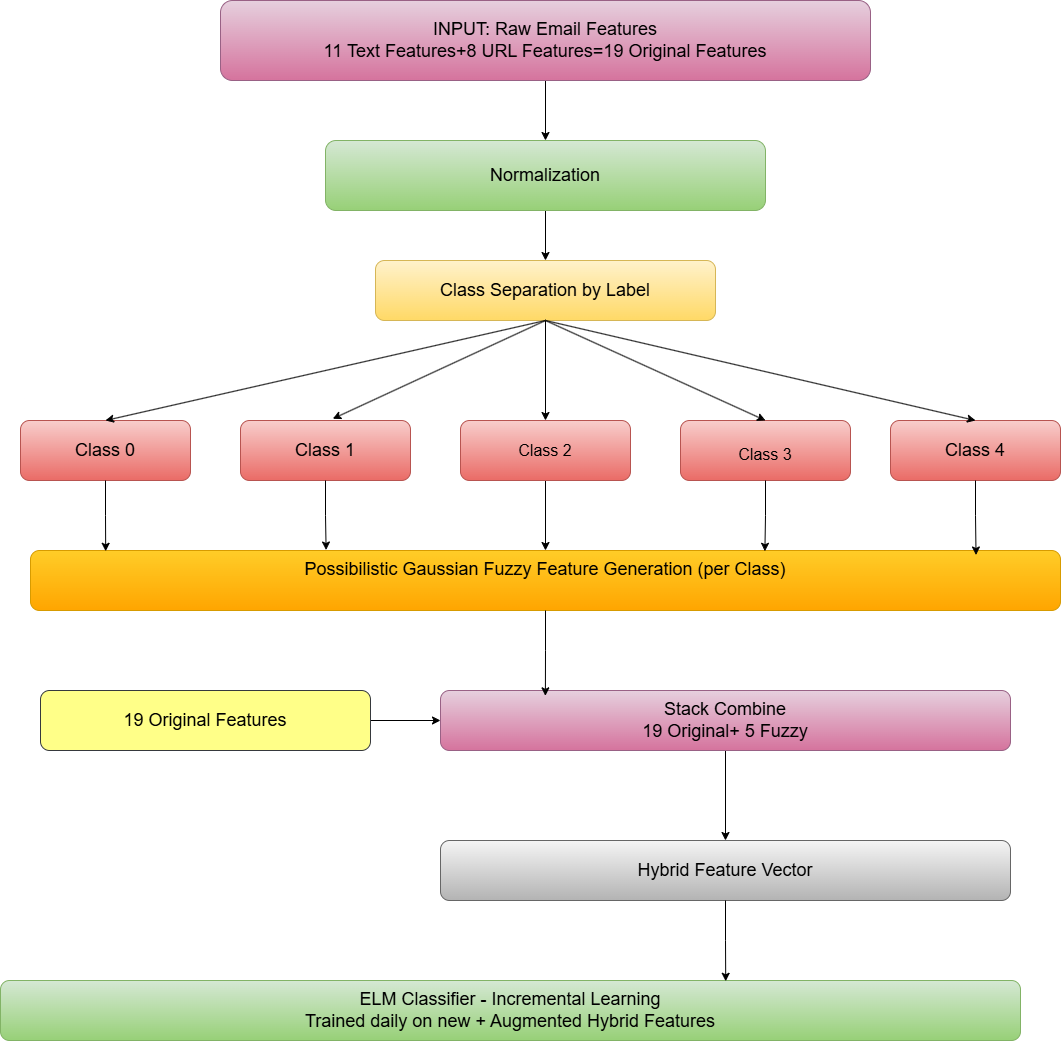
\includegraphics[width=\textwidth]{images/workflow_diagram.png}
    \caption{PGFDG-Based Feature Extraction}
    \label{fig:Fuzzy}
\end{figure}

Other features are: {Subspace Memberships} (computed on feature subsets), {Homogeneity}(relationship with class mean), {Outlier Score} (computed using modified Z-score and median absolute deviation), {Stability} (distance to median), and {Fuzzy Entropy}.

Among the 16 fuzzy features, five most representative features—Typicality, Density Score, Homogeneity, Outlier Score, and Fuzzy Entropy—are selected and incorporated into the normalized manual features.

A correction is applied to ensure that the fuzzy features are stored in the correct order using boolean masking.

The PGFDG-based fuzzy modeling approach improves robustness by incorporating uncertainty, structural density, and anomalies to improve class separation and generalization capabilities in the incremental social engineering attack detection problem.The detailed procedure for generating the fuzzy descriptors is presented in Algorithm~\ref{alg:fuzzy_pgfdg}.\\

\begin{algorithm}
\caption{Fuzzy Probability-Guided Feature Descriptor Generator (Fuzzy-PGFDG)}
\label{alg:fuzzy_pgfdg}
\begin{algorithmic}[1]

\Require $X \in \mathbb{R}^{n \times 19}$, 
$y \in \mathbb{R}^{n}$, 
$k=5$, $\epsilon=10^{-6}$

\Ensure $H \in \mathbb{R}^{n \times 24}$

\State $\hat{X} \gets (X - \mu_X)/\sigma_X$

\For{each class $c \in \{1,\dots,C\}$}

    \State $X_c \gets \{\hat{x}_i : y_i=c\}$

    \State $\mu_c \gets \frac{1}{|X_c|} \sum \hat{x}_i$

    \State $\Sigma_c \gets
    \frac{1}{|X_c|-1}
    \sum (\hat{x}_i-\mu_c)(\hat{x}_i-\mu_c)^T
    + \epsilon I$

    \State $M_c \gets \text{median}(X_c)$
    \State $\text{MAD}_c \gets \text{median}(|\hat{x}_i-M_c|)$

    \State $r_c \gets
    \text{percentile}_{25}
    (\|\hat{x}_i-\mu_c\|_2)$

\EndFor

\For{each sample $\hat{x}_i$}

    \State $d_M \gets
    \sqrt{(\hat{x}_i-\mu_c)^T
    \Sigma_c^{-1}
    (\hat{x}_i-\mu_c)}$

    \State $T_c \gets
    \exp\!\left(-\frac{1}{2} d_M^2\right)$

    \State $D_c \gets
    \frac{
    |\{x_j \in X_c :
    \|x_j-\hat{x}_i\|_2 \le r_c\}|
    }{|X_c|}$

    \State $\mathcal{H}_c \gets
    \frac{\hat{x}_i \cdot \mu_c}
    {\|\hat{x}_i\|_2 \|\mu_c\|_2}$

    \State $O_c \gets
    \min\!\left(
    1.0,
    \frac{0.6745\|\hat{x}_i-M_c\|_2}
    {\|\text{MAD}_c\|_2+\epsilon}
    \right)$

    \State $t \gets T_c$
    \State $\bar{t} \gets 1-t$

    \State $E_c \gets
    -t\log_2(t+\epsilon)
    -\bar{t}\log_2(\bar{t}+\epsilon)$

    \State $\phi_i \gets
    [T_{y_i},D_{y_i},
    \mathcal{H}_{y_i},
    O_{y_i},E_{y_i}]$

\EndFor

\State $F \gets [\phi_1|\dots|\phi_n]^T$

\State Select top $k$ least-correlated fuzzy features

\State $H \gets [\hat{X}\;|\;F_{\mathcal{S}}]$

\State \Return $H$

\end{algorithmic}
\end{algorithm}

\FloatBarrier
\subsection{Data Augmentation}

For the purpose of reducing the effects of class imbalance and catastrophic forgetting in the incremental learning framework, a supervised DAIL (Deterministic Alternating Interleaving Logic) data augmentation approach is proposed. The proposed approach uses the learned clusters of previous tasks to favor past class patterns when new data samples arrive.

As shown in ~\ref{fig:Data_aug}, the augmentation procedure is dependent on the hybrid features derived from the previous training phases. The data points are categorized based on their cluster labels, and for each category, the major class label is determined. The number of data points to be generated for the augmentation procedure is regulated by an augmentation ratio parameter $\alpha$, which determines the ratio of the augmentation procedure to the number of new data points entering the system. The number of augmentations is limited to enable proper pairing.

The synthetic instances are created through an alternating interleaving mechanism of features. Two parent instances are randomly chosen from the same cluster. The synthetic instances are created through an alternating fashion of choosing feature values from the two parent instances, where even-indexed features are chosen from one parent instance and odd-indexed features are chosen from the other parent instance, and then switched for the second synthetic instance. This deterministic interleaving process ensures that the characteristics of the class are maintained while new combinations of feature patterns are created. Since both parent instances belong to the same cluster, the labels are maintained.

\begin{figure}[H]
    \centering
    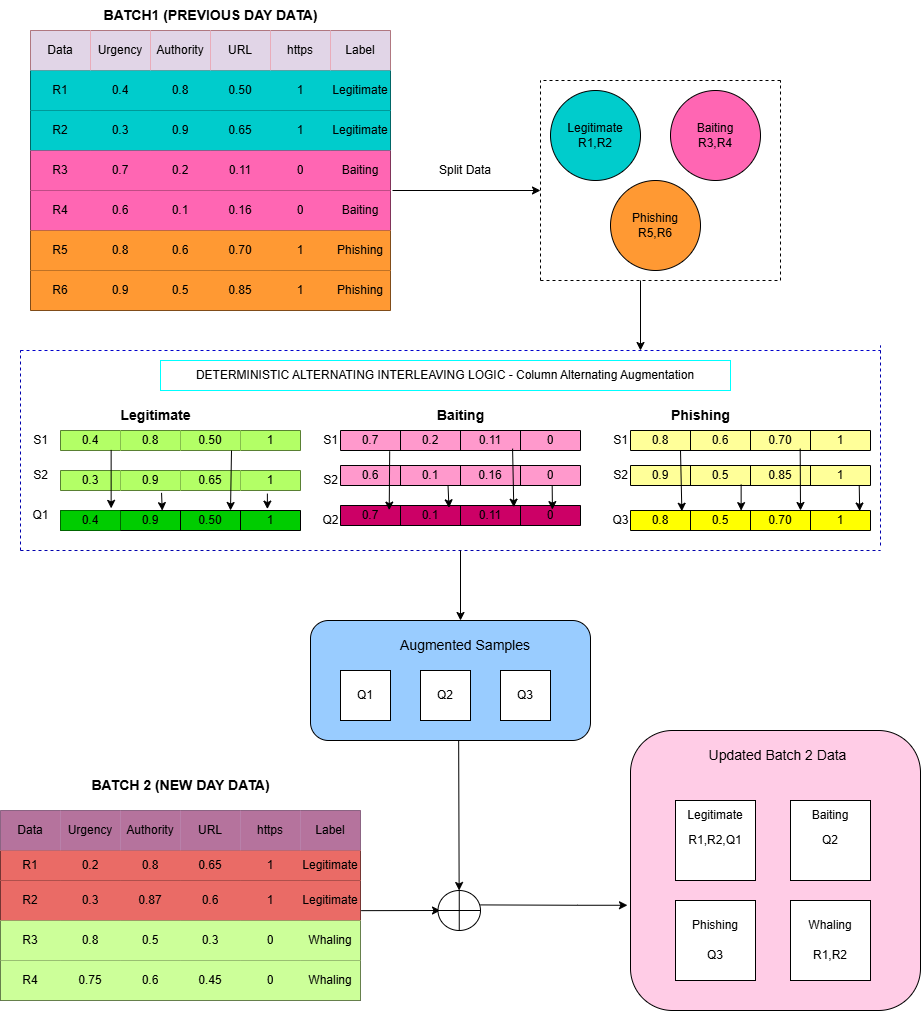
\includegraphics[width=\textwidth]{images/FYP_Augmentation.png}
    \caption{Data Augmentation- Column Alternating Approach}
    \label{fig:Data_aug}
\end{figure}

Each synthesized example is then labeled with the strongest class label from its source cluster, and the cluster labels are kept. The method obtains the expanded feature matrix, class labels, cluster labels, and a summary of the number of synthesized examples per class.

In conclusion, the DAIL method is a simple and supervised augmentation technique for controlled synthetic data generation. The method assists in preserving class distributions from previous learning without storing the whole past data, thus facilitating stable incremental learning and improving model robustness for dynamic social engineering attack detection.The detailed procedure of the DAIL augmentation process is presented in Algorithm~\ref{alg:dail}.

\begin{algorithm}[H]
\caption{DAIL Column-Alternating Augmentation}
\label{alg:dail}
\begin{algorithmic}

\Require 
$S^{(d-1)} \in \mathbb{R}^{m \times 124}$, 
$y^{(d-1)} \in \mathbb{R}^{m}$, 
$\mathrm{CID}^{(d-1)} \in \mathbb{R}^{m}$, 
$X_{\text{new}}^{(d)} \in \mathbb{R}^{p \times 124}$, 
$\alpha$, $K$

\Ensure 
$X_{\text{total}}^{(d)} \in \mathbb{R}^{(p+q)\times124}$, 
$y_{\text{total}}^{(d)} \in \mathbb{R}^{p+q}$

\State \textbf{Phase 1: Per-Cluster Augmentation Budget}

\State $n_{\text{budget}} \gets \alpha \cdot p$

\For{$k = 1$ to $K$}
    \State $S_k \gets \{ s_i \in S^{(d-1)} : \mathrm{CID}_i = k \}$
    \State $n_k \gets |S_k|$
    \State $n_k^{\text{aug}} \gets 
    \min\!\left(\left\lfloor\frac{n_k}{2}\right\rfloor,
    \left\lfloor\frac{n_{\text{budget}}}{K}\right\rfloor\right)$
    \State $n_k^{\text{aug}} \gets n_k^{\text{aug}} - 
    (n_k^{\text{aug}} \bmod 2)$
\EndFor

\Statex
\State \textbf{Phase 2: Column-Alternating Generation}

\State $X_{\text{aug}} \gets \emptyset$, 
$y_{\text{aug}} \gets \emptyset$

\For{$k = 1$ to $K$}

    \State $\{ s_1, s_2, \dots, s_{n_k^{\text{aug}}} \} 
    \gets$ random samples from $S_k$ (without replacement)

    \For{$i = 1,3,5,\dots,n_k^{\text{aug}}-1$}

        \For{$j = 0$ to $123$}

        \[
        Q_1[j] =
        \begin{cases}
        s_i[j] & \text{if } j \bmod 2 = 0 \\
        s_{i+1}[j] & \text{if } j \bmod 2 = 1
        \end{cases}
        \]

        \[
        Q_2[j] =
        \begin{cases}
        s_{i+1}[j] & \text{if } j \bmod 2 = 0 \\
        s_i[j] & \text{if } j \bmod 2 = 1
        \end{cases}
        \]

        \EndFor

        \State $y_{Q_1} = y_{Q_2} \gets 
        \mathrm{mode}(\{ y_i : \mathrm{CID}_i = k \})$

        \State $X_{\text{aug}} \gets 
        X_{\text{aug}} \cup \{Q_1, Q_2\}$

        \State $y_{\text{aug}} \gets 
        y_{\text{aug}} \cup \{y_{Q_1}, y_{Q_2}\}$

    \EndFor
\EndFor

\Statex
\State \textbf{Phase 3: Merge}

\State $X_{\text{total}}^{(d)} \gets 
\begin{bmatrix}
X_{\text{new}}^{(d)} \\
X_{\text{aug}}
\end{bmatrix}$

\State $y_{\text{total}}^{(d)} \gets 
\begin{bmatrix}
y_{\text{new}}^{(d)} \\
y_{\text{aug}}
\end{bmatrix}$

\Statex
\State \textbf{Phase 4: Memory Cleanup}

\State Delete $S^{(d-1)}$, Delete $\mathrm{ELM}^{(d-1)}$
\State $S^{(d)} \gets X_{\text{total}}^{(d)}$

\State \Return $X_{\text{total}}^{(d)}, y_{\text{total}}^{(d)}$

\end{algorithmic}
\end{algorithm}


\subsection{ELM Classifier}

The Extreme Learning Machine (ELM) classifier provides an extremely efficient method for training a neural network classifier compared to the standard training method. Unlike the MLP classifier, which needs to be trained using the backpropagation method, the ELM classifier initializes the weights and biases of the hidden layers randomly and keeps them fixed throughout the entire training process. This reduces the computational overhead involved in training a neural network classifier. Once the transformation of the hidden layers is determined, the ELM classifier computes the output weights in one step, allowing for extremely fast training.

Given an input matrix \(X \in \mathbb{R}^{N \times 150}\) and the corresponding output label matrix \(Y \in \mathbb{R}^{N \times K}\), the hidden layer output of ELM is computed as

\begin{equation}
H = \sigma\!\left(\mathbf{1}\beta_0 + XW\right)
\end{equation}

where \(W \in \mathbb{R}^{150 \times L}\) is a randomly initialized weight matrix, \(\beta_0 \in \mathbb{R}^{1 \times L}\) is a random bias row vector, \(L\) is the number of hidden neurons (here \(L=150\)), and \(\mathbf{1}\in\mathbb{R}^{N\times 1}\) is a column vector of ones used to broadcast the bias across \(N\) rows. The activation \(\sigma\) is the sigmoid function:

\begin{equation}
\sigma(x) = \frac{1}{1 + e^{-x}}
\end{equation}


This activation function projects the actual inputs to the range \((0,1)\), which helps the hidden layer to produce a smooth non-linear projection of the fused features. Since \(W\) and \(\beta_0\) are random variables and are fixed, the hidden layer can be treated as a feature projector that projects the input into an informative representation very quickly.

Once the hidden layer output matrix \(H\in\mathbb{R}^{N\times L}\) is obtained, the output weights \(\beta\in\mathbb{R}^{L\times K}\) are computed analytically using the Moore–Penrose pseudoinverse:

\begin{equation}
\beta = H^{\dagger}Y
\end{equation}

with one common expression for the pseudoinverse (when \(H^{T}H\) is invertible) given by

\begin{equation}
H^{\dagger} = (H^{T}H)^{-1}H^{T}
\end{equation}


This provides the least squares solution that directly relates the features of the hidden layers to the desired outputs in a single linear solve. However, in practice, to improve numerical stability, especially when \(H^{T}H\) is close to being singular, a regularized solution is usually used:

\begin{equation}
\beta = \left(H^{T}H + \lambda I\right)^{-1} H^{T} Y
\end{equation}

where \(\lambda>0\) is a small regularization parameter and \(I\) is the \(L\times L\) identity matrix.

With the application of this analytical training method, the ELM classifier is able to efficiently learn the decision boundaries based on the combined latent features obtained from the Stacked Autoencoders. This is particularly useful in scenarios that require rapid model training or system update. The complementary nature of the ELM classifier with the MLP classifier further enhances the robustness of the system, which is capable of rapid and precise identification of various patterns of social engineering attacks.

As shown in Algorithm~\ref{alg:ELM}, the Extreme Learning Machine computes the hidden layer outputs and the output weights analytically.


\begin{algorithm}[H]
\caption{Algorithm for Extreme Learning Machine (ELM)}
\label{alg:ELM}
\begin{algorithmic}[1]


\State \textbf{Input:} Training feature matrix $X$, label vector $Y$, number of hidden neurons $N_h$, activation function

\State Randomly initialize hidden layer weights $W_h$ and biases $b_h$

\State Compute hidden layer output matrix $H$:
\For{each sample $x_i$ in $X$}
    \State $h_i = activation(W_h \cdot x_i + b_h)$
\EndFor

\State Compute output weights $\beta$ using Moore--Penrose pseudoinverse:
\State $\beta = pinv(H) \cdot Y$

\State \textbf{Training complete:} ELM model is ready after obtaining $\beta$

\State \textbf{Prediction:} For a new sample $x_{\text{new}}$:
\State $h_{\text{new}} = activation(W_h \cdot x_{\text{new}} + b_h)$
\State Output label prediction: $y_{\text{new}} = h_{\text{new}} \cdot \beta$

\end{algorithmic}
\end{algorithm}
\subsection{Incremental Learning}

The proposed system uses a structured four-day incremental learning method to simulate the occurrence of social engineering attack types in the real world. Instead of training a single model, the classifier is updated as new classes and samples are added. This method enables the system to adapt continuously without catastrophic forgetting.

On Day 1, the training of the model is performed on the first three classes: Legitimate, Phishing, and Baiting. A fixed number of samples for each class are selected to form the initial training set. The hybrid feature extraction is performed by the stacked autoencoder (Pipeline 1) and fuzzy PGFDG features (Pipeline 2), resulting in a 124-dimensional feature space. The dataset is split using an 80/20 stratified train-test split, and an Extreme Learning Machine (ELM) classifier is trained. The number of hidden neurons is dynamically adjusted as $200 \times n_{\text{classes}}$, which is adjusted based on the number of classes.

On Day 2, new samples are added from selected classes. Instead of retraining the model from scratch, the approach includes supervised DAIL augmentation using the stored Day 1 features. New samples are created cluster-wise and combined with the new incoming samples. The pool of samples is then divided and used to train a new ELM model. After the successful training of the model, the old model instance is deleted to save memory.

On Day 3, a new class (Pretexting) is introduced, thus adding to the number of classes in the classification task. Once again, the same procedure is followed: new data is passed through frozen encoders from Day 1 to maintain consistency in the feature space, DAIL augmentation is performed based on the representations from Day 2, and a new ELM is learned. The size of the hidden layer is automatically determined based on the new number of classes.

On Day 4, all five classes (Legitimate, Phishing, Baiting, Whaling, and Pretexting) are trained together. New data is combined with the learned features from Day 3, and a new ELM is trained. Confusion matrix and test accuracy are computed to check the performance. In all stages, the feature encoders are frozen after Day 1 to ensure a fixed feature space.

This incremental learning approach has several advantages. Firstly, it is possible to incrementally add new attack types without the need to retrain on the whole past data. Secondly, the supervised DAIL learning approach assists in reinforcing past class distributions learned by the model, hence combating catastrophic forgetting. Thirdly, the dynamic scaling of hidden neurons assists the ELM classifier in adapting to the increasing complexity of the classes. Finally, past model copies are deleted after each update, hence promoting efficient memory use.

The incremental learning approach hence assists in adaptive, scalable, and memory-efficient social engineering attack detection.
